\section{Estado del Arte y Antecedentes}

\subsection{2.1 Evolución de AM en Sector Aeroespacial}

Resulta revelador observar cómo la fabricación aditiva ha transitado en poco más de una década desde aplicaciones marginales en prototipado hasta convertirse en una tecnología estratégica para sistemas espaciales. Aunque los enfoques terrestres tradicionales siguen dominando la producción en serie, la necesidad de minimizar masa y maximizar funcionalidad ha impulsado su adopción en entornos de alta exigencia.

Uno de los giros más interesantes en esta evolución consiste en la exploración de manufactura in-situ. Jonckers et al. propusieron el concepto de satélites free-flying capaces de fabricar estructuras grandes directamente en órbita, una idea que contrasta fuertemente con los paradigmas actuales de lanzamiento completo desde Tierra \cite{Jonckers2022}. Este enfoque promete reducir drásticamente las restricciones impuestas por las vibraciones de lanzamiento y las limitaciones de tamaño de carenados, aunque todavía enfrenta desafíos importantes de precisión y control en microgravedad. En muchos casos estudiados, las implementaciones terrestres de AM han demostrado mayor madurez, especialmente en aleaciones de aluminio, titanio y materiales poliméricos avanzados.

No obstante, cabe matizar que la calificación espacial sigue siendo un cuello de botella. La variabilidad inherente de los procesos aditivos exige protocolos de certificación más rigurosos que los métodos sustractivos, lo cual ralentiza su integración en misiones de alto valor.

\subsection{2.2 Aplicaciones en Antenas y RF para SATCOM}

Particularmente llamativo es el salto cualitativo que ha experimentado la fabricación aditiva cuando se aplica a componentes de radiofrecuencia para comunicaciones satelitales. Lejos de ser un asunto resuelto, el diseño de antenas y alimentadores en bandas Ku y Ka exige compromisos complejos entre ganancia, ancho de banda, masa y disipación térmica.

Talpur et al. ofrecen en su revisión sistemática una cartografía detallada de las principales técnicas empleadas \cite{Talpur2025}. Mientras la Fused Deposition Modeling (FDM) destaca por su bajo costo y rapidez en prototipos, tiende a mostrar limitaciones en acabado superficial y estabilidad térmica. Por otro lado, la Powder Bed Fusion (DMLS/SLM) permite obtener estructuras metálicas con excelente conductividad y geometrías internas optimizadas, aunque a un costo energético y de post-procesado superior. La Stereolithography (SLA) con resinas metalizables ocupa un espacio intermedio interesante para arrays y reflectores.

En muchos casos estudiados, los componentes AM logran reducir masa entre 30\% y 50\% respecto a sus equivalentes mecanizados, además de integrar funciones de guía de onda y disipación térmica en una sola pieza. Estas ventajas resultan especialmente valiosas en constelaciones LEO donde el costo por kilogramo lanzado sigue dictando viabilidad económica.

\begin{table}[h]
\centering
\caption{Comparación de tecnologías de fabricación aditiva para componentes RF satelitales}
\label{tab:tecnologias_am}
\begin{tabular}{lcccc}
\hline
\textbf{Tecnología} & \textbf{Materiales típicos} & \textbf{Resolución} & \textbf{Ventajas principales} & \textbf{Limitaciones} \\
\hline
FDM & Polímeros, composites & Media & Bajo costo, rapidez & Acabado superficial \\
SLA & Resinas fotopolimerizables & Alta & Detalle fino & Propiedades mecánicas \\
DMLS/SLM & Al, Ti, Acero inoxidable & Alta & Alta conductividad & Costo y distorsión térmica \\
Binder Jetting & Cerámicos, metales & Media-Alta & Escalabilidad & Post-procesado extenso \\
\hline
\end{tabular}
\end{table}

\subsection{2.3 Casos de Estudio en Plataformas Satelitales}

Uno de los ejemplos más consistentes de optimización estructural mediante AM proviene del rediseño de plataformas satelitales. Boschetto et al. aplicaron estructuras lattice internas y thickening selectivo en componentes primarios fabricados por PBF-LB/M, consiguiendo reducciones de masa significativas sin comprometer el comportamiento modal bajo cargas dinámicas de lanzamiento \cite{Boschetto2023}. Su trabajo ilustra con claridad cómo el Design for Additive Manufacturing (DfAM) permite ir más allá de la mera ligereza, logrando piezas multifuncionales que integran interfaces mecánicas y canales térmicos.

Estos casos revelan un patrón recurrente: la consolidación de ensamblajes complejos en una o pocas piezas reduce drásticamente puntos de fallo potenciales y tiempos de integración. Sin embargo, la literatura también pone de manifiesto limitaciones persistentes relacionadas con anisotropía de propiedades, acabados superficiales y la necesidad de extensas campañas de prueba.

\begin{figure}[h]
\centering
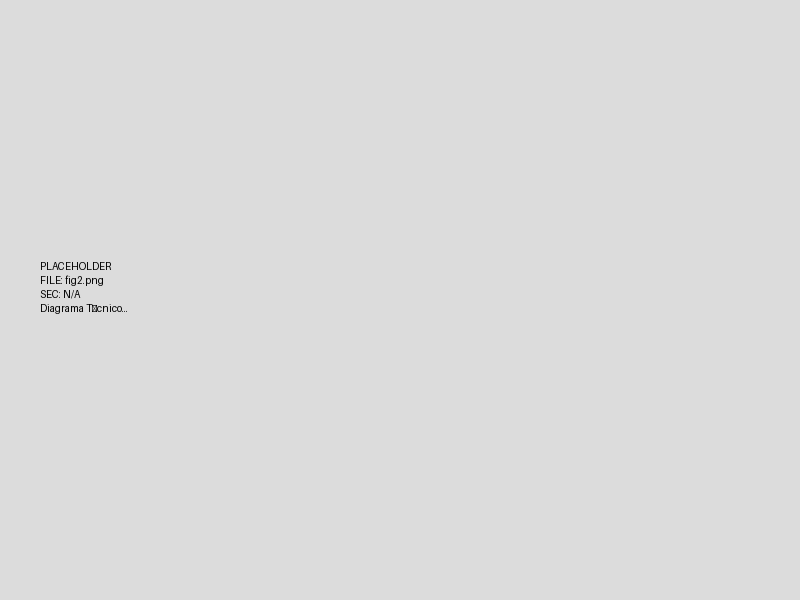
\includegraphics[width=0.9\linewidth]{fig2.png}
\caption{Ejemplos representativos de componentes fabricados aditivamente: bracket estructural lattice y antena RF integrada para aplicaciones SATCOM. Se destacan las geometrías internas optimizadas imposibles de obtener mediante mecanizado convencional.}
\label{fig:ejemplos_brackets_antenas}
\end{figure}

En conjunto, el estado del arte muestra un claro avance hacia la madurez, aunque persisten brechas importantes entre demostraciones en laboratorio y despliegue en misiones operativas de telecomunicaciones a gran escala. Esta realidad marca el punto de partida para la metodología que se desarrolla en las siguientes secciones.